\documentclass[output=paper, modfonts]{langscibook} 
\ChapterDOI{10.5281/zenodo.6393732}

\title{Velar Tap in Dàgáárè}  

\author{Samuel Akinbo\affiliation{University of British Columbia} and  Alexander Angsongna\affiliation{University of British Columbia} and Avery Ozburn\affiliation{University of British Columbia} and Murray Schellenberg\affiliation{University of British Columbia} and Douglas Pulleyblank\affiliation{University of British Columbia}}


\abstract{\citet{bodomo1997} describes intervocalic velar [g] in Dàgáárè as fricative [ɣ]. With 42 tokens of intervocalic [g] from a native speaker of Dàgáárè, we investigated the acoustic and articulatory features of the Dàgáárè intervocalic velar [g] using ultrasound images, waveforms, spectrograms, and palatogram. The results of the study suggest that  Dàgáárè intervocalic [g] is not a fricative but a velar with strong tap-like features, a previously unattested sound in natural language \citep{ladefoged1990revised}. Following from this, we conclude that Dàgáárè intervocalic velar [g] is not a fricative but a tap.}

\begin{document}
\graphicspath{{figures/}}
\SetupAffiliations{mark style=none}
\lehead{Samuel Akinbo et al.}
\maketitle

\section{Introduction} 
D\`ag\'a\'ar\'e is a Gur language of the Niger-Congo family, part of a languages group known as the Mabia languages. It is spoken by about 1.5 million people in northwestern Ghana and some parts of Burkina Faso \citep{kennedy1966collected, bodomo1997}.

Dàgáárè is described as having twenty-five consonants and two underlying glides \citep{bodomo1997}. The vowel inventory contains nine vowels, with tongue root contrasts for high and mid vowels, but a single low vowel [a]. In Bodomo's (\citeyear{bodomo1997}) description of the consonant inventory, the voiced velar stop [g] is said to alternate with [ɣ] intervocalically. The data included with this description is the single word (/p\'ɔg\'ɔ/ ‘woman’) where [g] occurs between RTR vowels. According to our auditory impression, including that of the second author who is a native speaker, intervocalic <g> is not a velar fricative.

This paper describes an acoustic and articulatory study of Dàgáárè <g> in Central Dàgáárè, spoken in Nadowli-Kaleo district in Ghana. Waveforms, spectrograms, duration, ultrasound images, and static palatograms of intervocalic <g> are studied. The acoustic and articulatory results show that intervocalic <g> has the complex waveform, amplitude variation, formant structure, tongue movement, and closure typical of a tap, rather than a velar fricative.
 

\section{Methodology}
The data come from a native speaker of Dàgáárè and was collected at ISRL Lab, University of British Columbia, in a room using Sennheiser MKH\,8060 shotgun microphone at the sampling rate of 44kHz/16bit.

An Aloka Pro-Sound SSD\,5000 ultrasound machine with an Aloka UST-9119-3.5 convex transducer (pulse frequency 3.5MHz, field of view 120º) collected a moving image of tongue movement. The ultrasound probe was positioned manually against the mylohyoid muscle and was kept stable with a mechanical arm. The stimuli for ultrasound and acoustic studies contain 42 tokens with intervocalic [g]. Each token was repeated twice.

\begin{sloppypar}
To determine the place of articulation of the closure, a palatogram was recorded. The tongue was painted with charcoal mixed in olive oil before the participant produced four tokens with intervocalic <g>. After articulating each of the tokens, an image of the soft-palate was captured.
\end{sloppypar}

\section{Results}
All instances of intervocalic <g> were segmented manually in Praat \citep{boersma2002praat} and a script was used to extract duration values. The waveform and spectogram were manually extracted.

The waveform of Dàgáárè <g> has an decrease in amplitude compared to surrounding vowels, but it is complex as can be seen in Figure \ref{tab:1:spectogram}. This is similar to the expected properties of a tap, but distinct from both voiced velar stops and resonants; from a voiced stop, we would expect a simple waveform for voicing, while with a resonant, we would not expect an amplitude decrease.

\begin{sloppypar}
In the spectrogram of Dàgáárè <g>, we regularly see formant structure throughout the consonant. This is typical of resonants and possible for taps but is not consistent with a stop. For a [g], we would expect a gap in the spectrogram with a voicing bar at the bottom; but this is not what we see for Dàgáárè <g>. With a fricative, we would expect random noise, which is again not what we see. the spectrogram also shows that <g> does not feature spectral energy like the other non-sibilant fricative [v] in the spectrogram or a dorsal fricative (see \citealt{jesus2005acoustic}).
\end{sloppypar}

\begin{figure}[H]
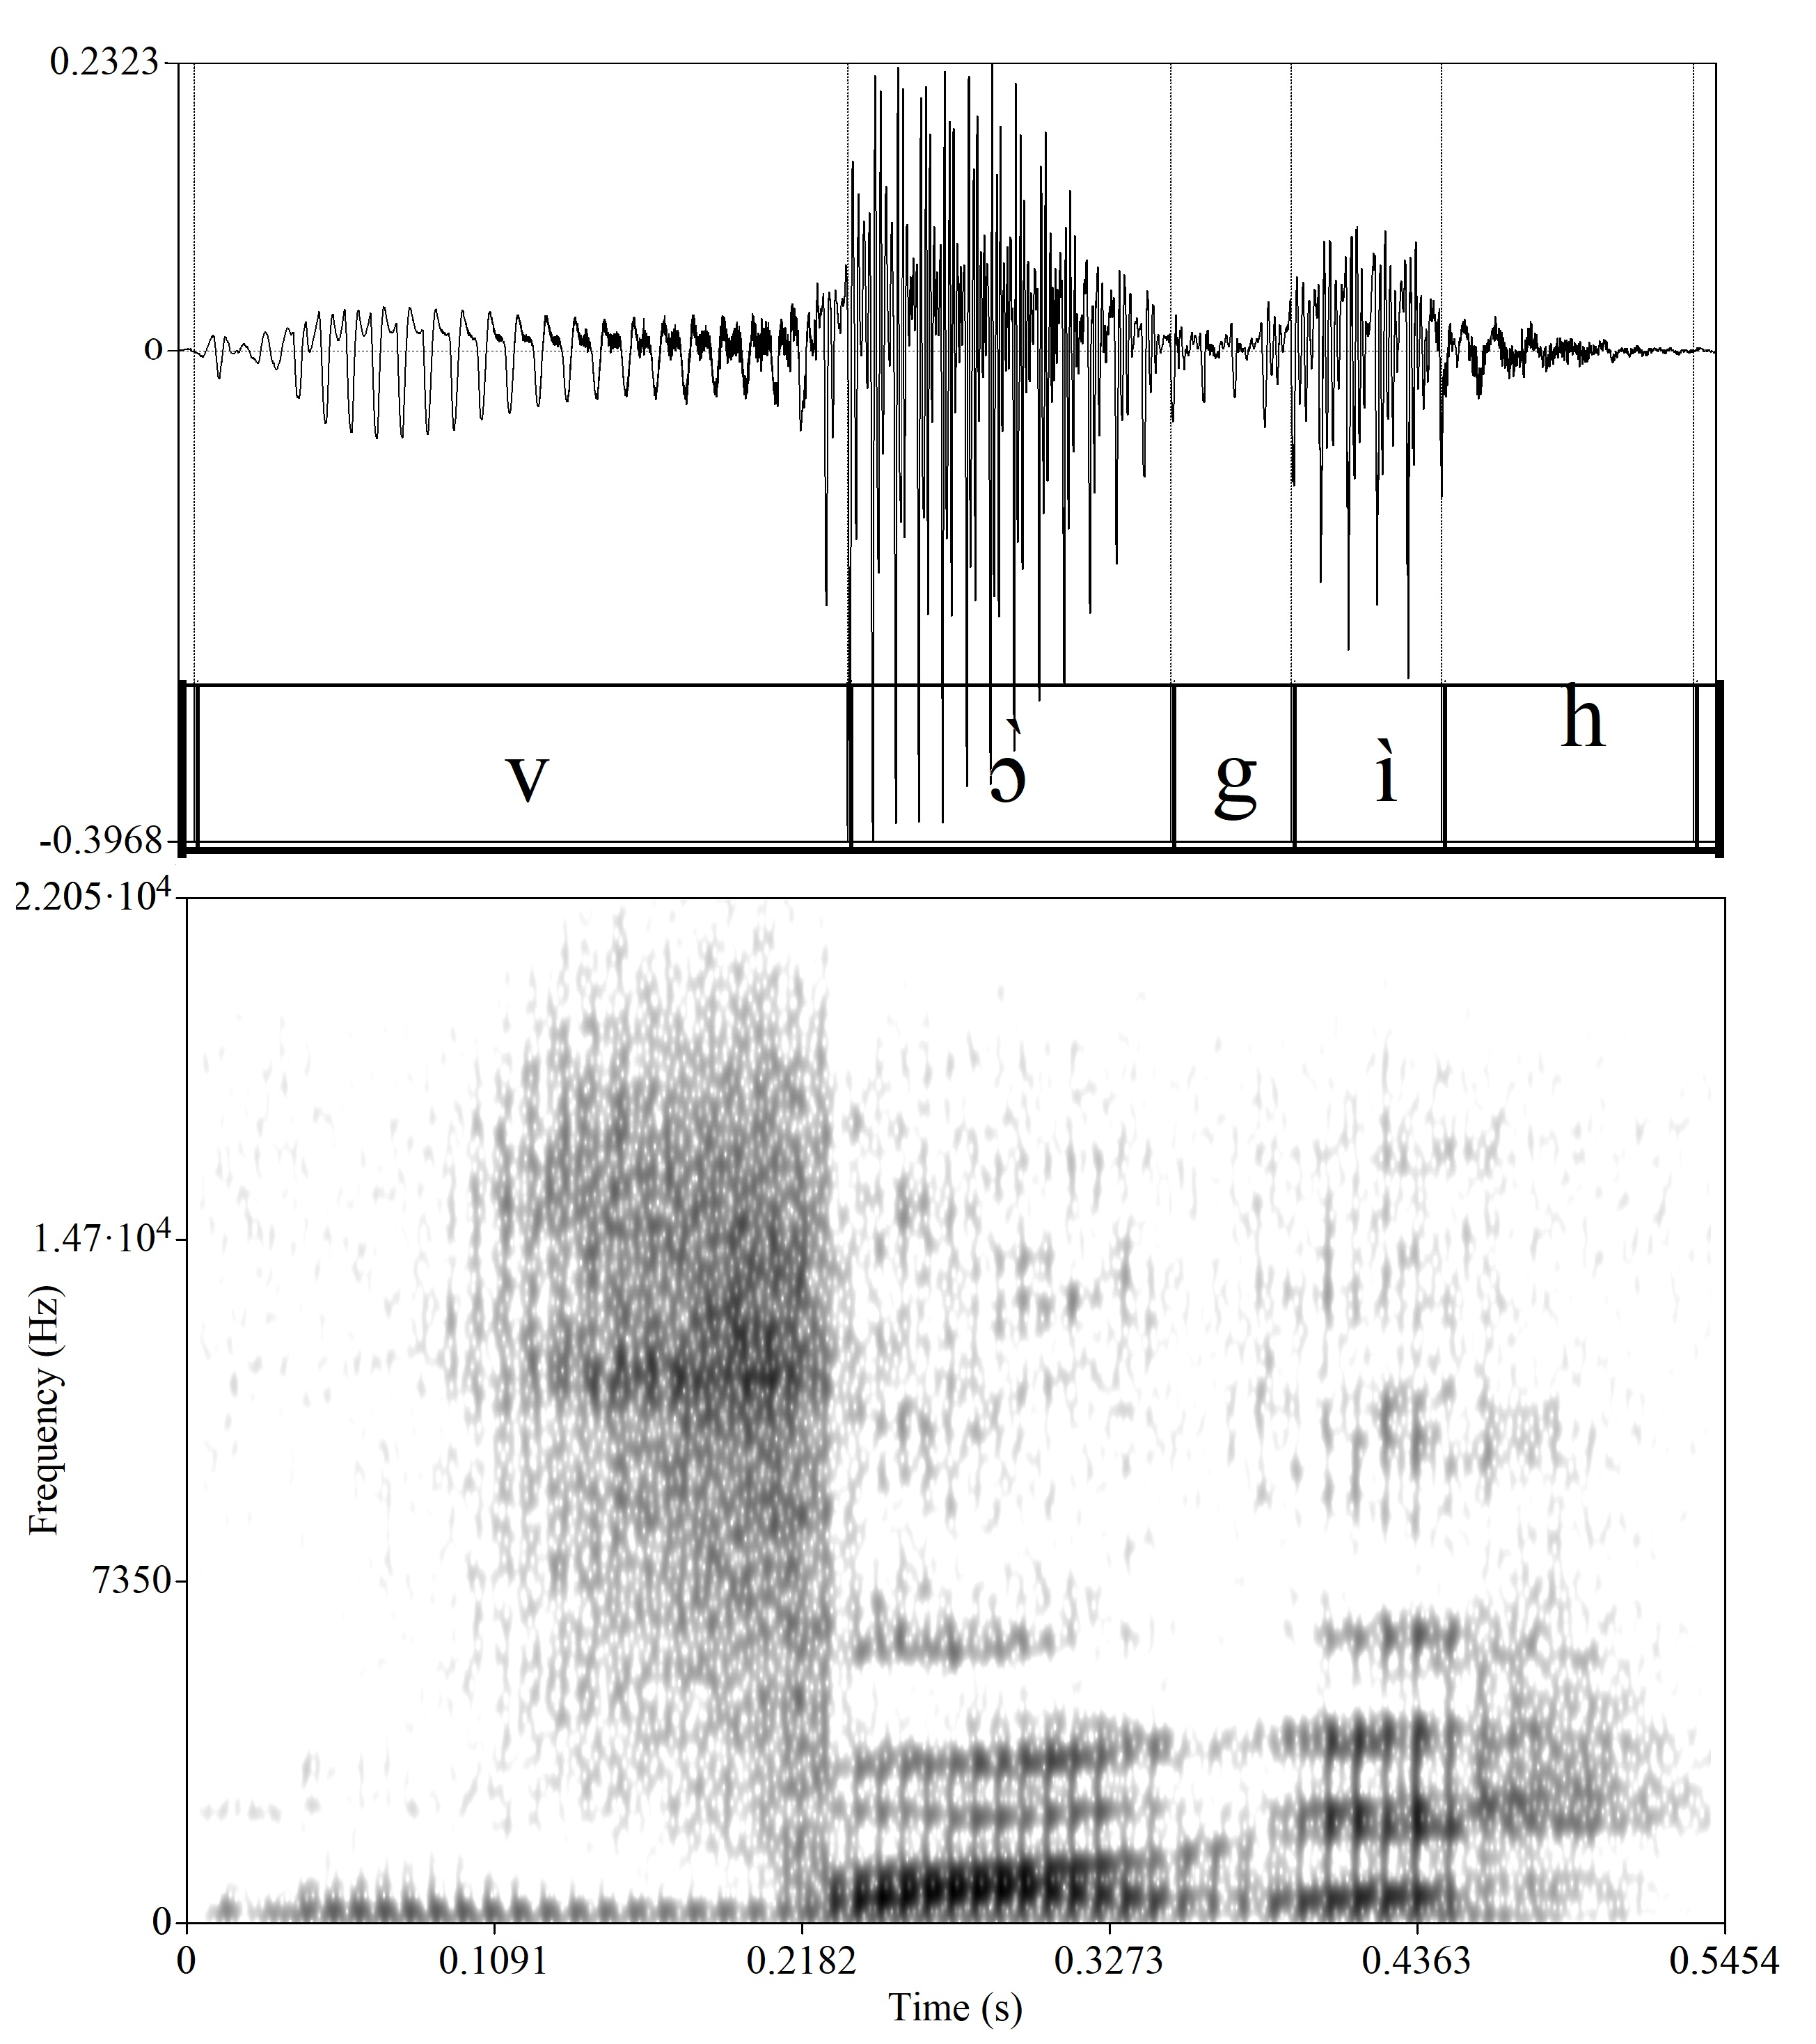
\includegraphics[width=0.75\linewidth]{wave_specto_vogi2.jpg}
  \caption{Waveform (top) and spectogram (bottom) of Dàgáárè <g>}
  \label{tab:1:spectogram}
\end{figure}


In terms of duration (including both closure duration and release duration), the average duration of the collected <g> tokens was 0.055 seconds. This is substantially shorter than English [g], as a comparison, which has a duration of around 0.081 seconds (\citealt{byrd199354}: closure duration 54ms, release duration 27ms). It is also longer than an alveolar tap, which tends to have a duration between 0.028 and 0.041 seconds. The durations for the Dàgáárè velar can be seen compared to English [g] and [ɾ] in Figure \ref{tab:2:duration}. 


On the ultrasound, the tongue movement between the vowel position and the consonant was substantial; the tongue back raised towards the palate/velum. This degree of movement is consistent with either a stop or a tap, because the tongue moves far from the vowel position to make closure. A resonant would have less movement, due to the lack of closure. The ultrasound images can be seen in Figure \ref{tab:3:ultrasound}. A fricative would have less movement than a stop or tap, but more than a resonant; these images are  potentially consistent with a fricative. 

\begin{figure}[p]
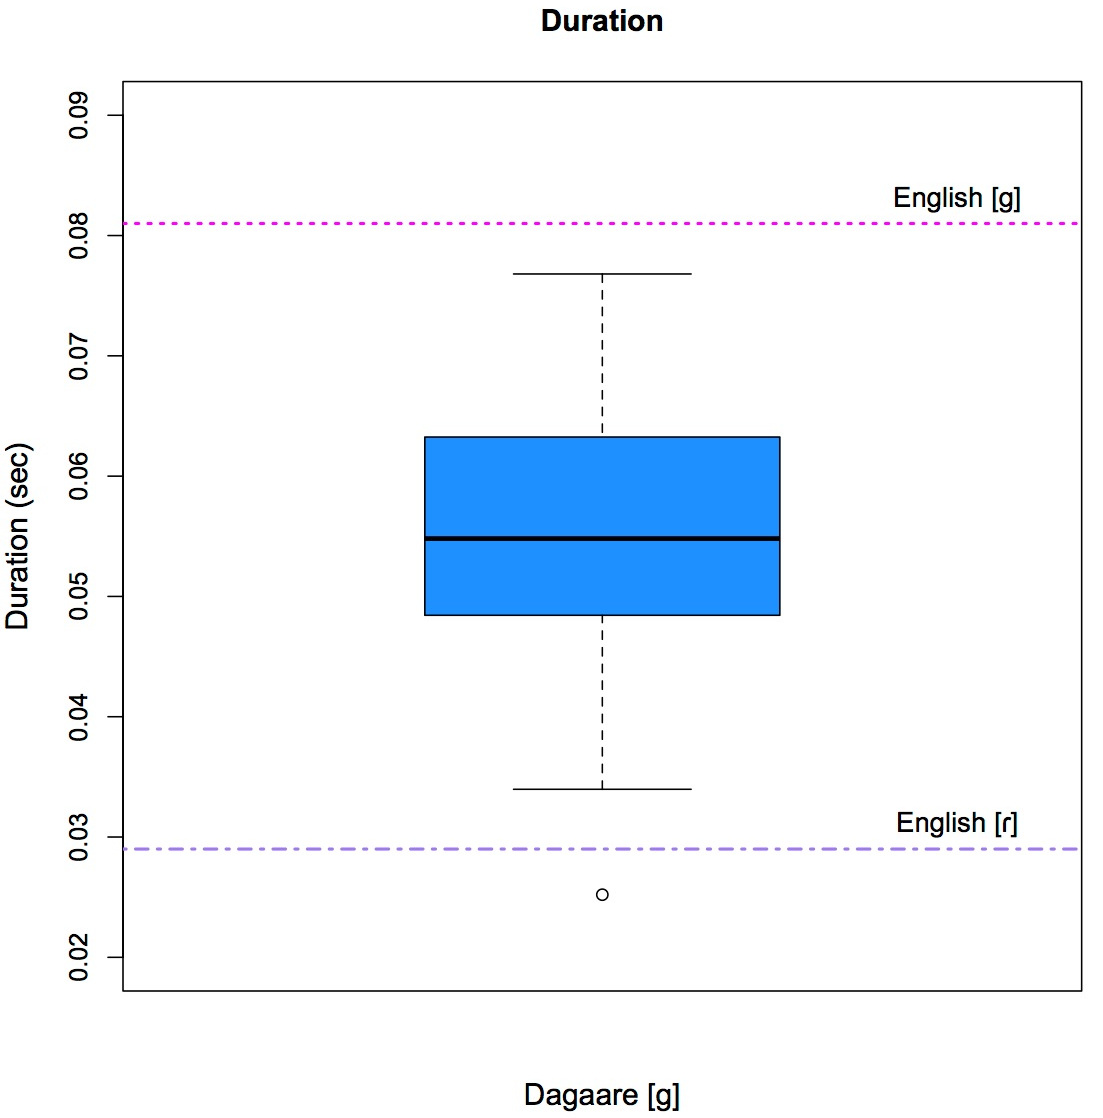
\includegraphics[width=.8\linewidth]{g_duration.jpg}
\caption{Dàgáárè <g> relative to English [g] and [ɾ]}
\label{tab:2:duration}
\end{figure}

\begin{figure}[p]
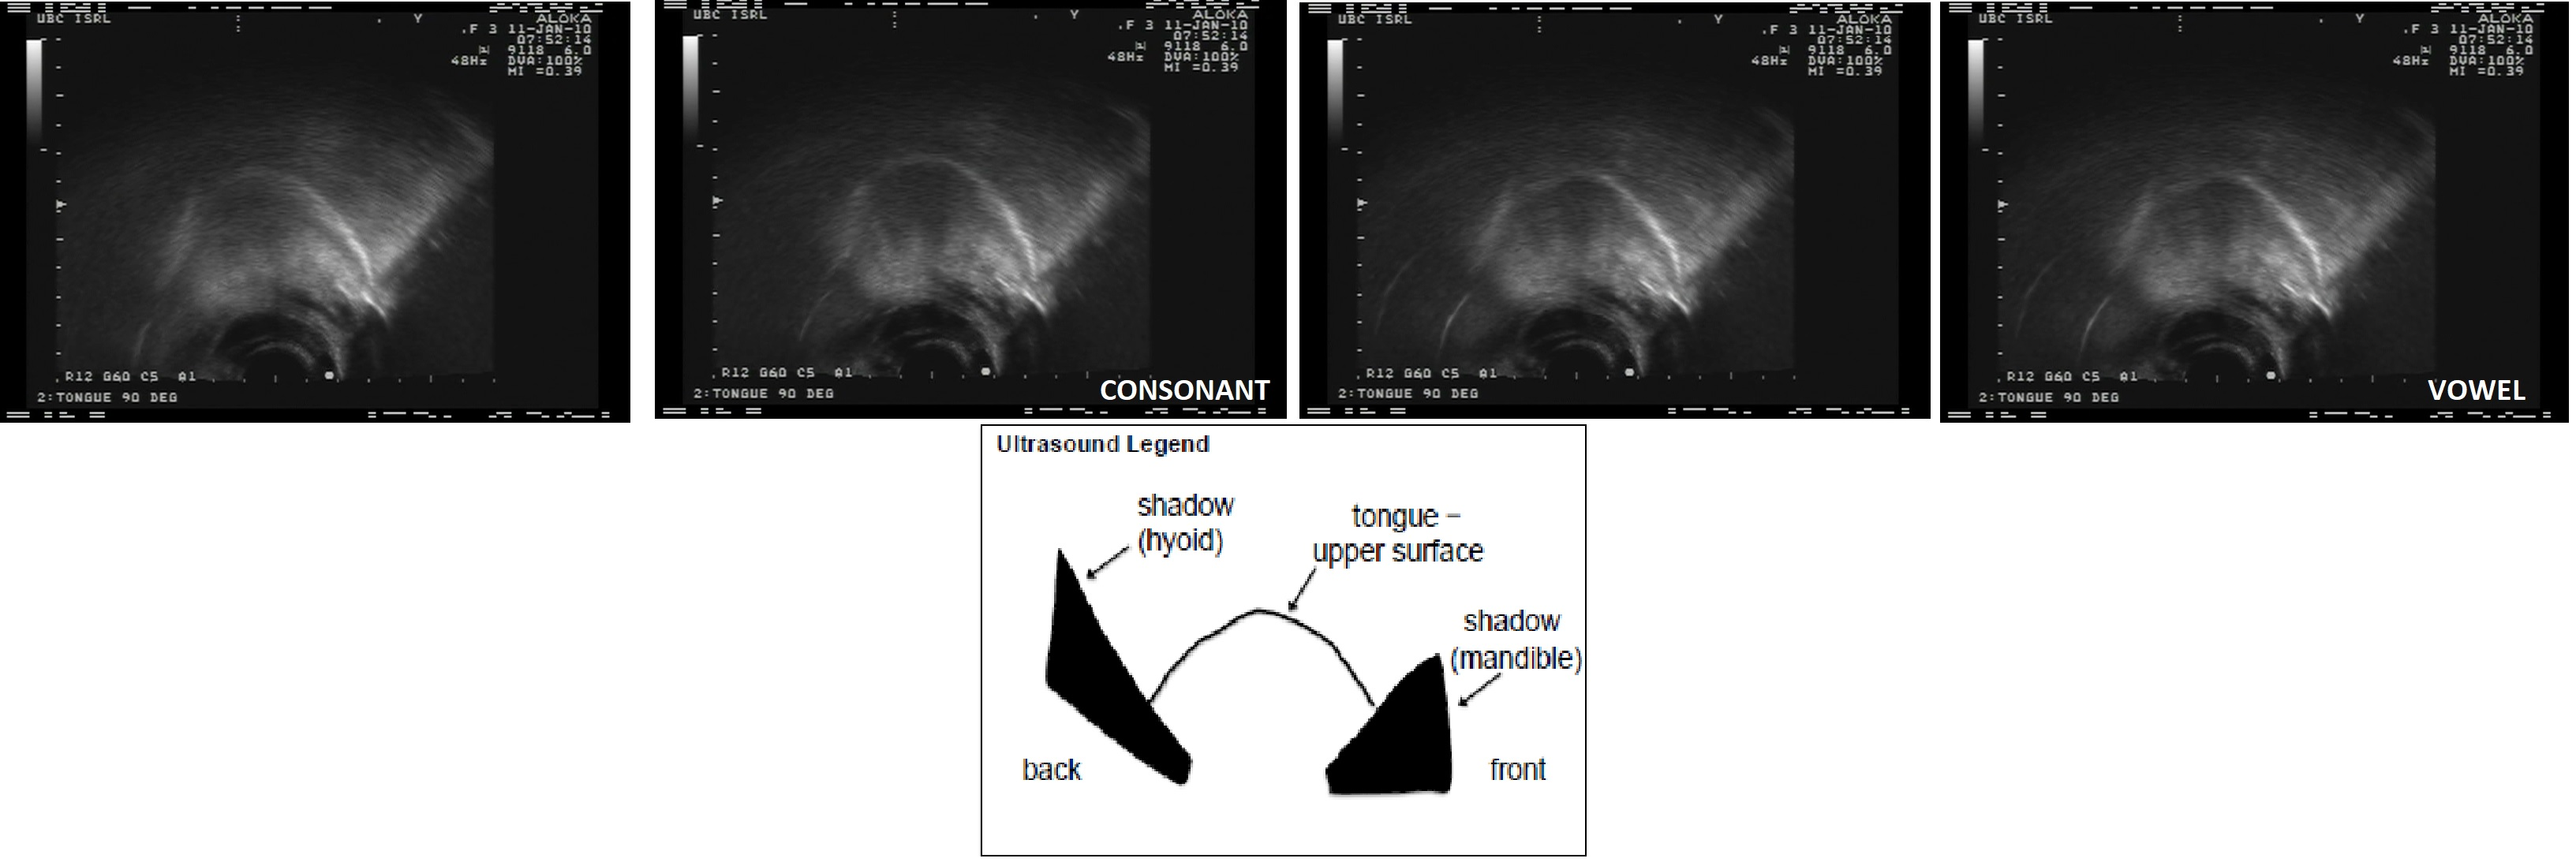
\includegraphics[width=1\linewidth]{ultrasound.jpg}
\caption{Intervocalic <g> in Dàgáárè}
\label{tab:3:ultrasound}
\end{figure}



In the palatography shown in Figure \ref{tab:4:palatogram} (page~\pageref{tab:4:palatogram}), the pattern of charcoal left on the palate after production of <g> showed evidence of closure in the palatal/velar region. Closure is typically seen for stops and taps, but not for resonants or fricatives.

In summary, although the  Dàgáárè <g> has a longer duration than an alveolar tap, its production is most consistent with the behaviour of a tap, in terms of waveform, spectrogram, ultrasound, and palatography. In particular, it is not consistent with a stop or a resonant in a number of ways. These results are summarized in Table \ref{tab:1:summary} (page~\pageref{tab:1:summary}).

\begin{figure}[p]
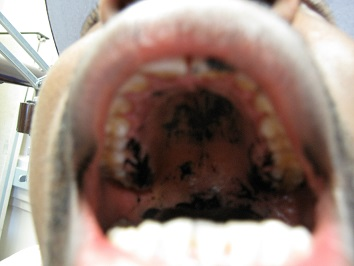
\includegraphics[width=0.5\linewidth]{palatograph.jpg}
\caption{Palatogram showing closure}
\label{tab:4:palatogram}
\end{figure}

\begin{table}[p]
\small
\caption{Result summary\label{tab:1:summary}}
 \begin{tabularx}{\textwidth}{l QQQQQ} 
  \lsptoprule
                &                           & \multicolumn{4}{c}{Expected of}\\\cmidrule(lr){3-6}
     Properties & {Dàgáárè results} & [g]\footnote{\citep{byrd199354}} & tap\footnote{\citep{ting2007understanding}} & resonant & fricative\\ 
  \midrule
  Waveform  &complex waveform, amplitude decrease & simple waveform (voicing) &  more complex waveform,
  amplitude decrease  &no amplitude decrease &random pattern in the waveform \\\tablevspace
  Spectogram  &  formant structure &  gap with voicing bar &    formant structure possible    & formant structure & random noise \\\tablevspace
  Duration  &  0.055 sec &   \~{}0.081 sec &\~{}0.028–0.041 sec    & <n/a> &<n/a> \\\tablevspace
  Ultrasound  &  lots of tongue movement &   lots of mvt. & lots of mvt.& less mvt. & intermed. mvt.\\\tablevspace
  Palatography  &  closure &  closure &    closure    & no closure &no closure \\
  \lspbottomrule
 \end{tabularx}
\end{table}



\section{Discussion and conclusion}
The results show that intervocalic [g] in Dàgáárè has a complex waveform, amplitude decrease, formant structure, a short duration, significant tongue movement, and closure. These features are strong tap-like features and suggest that Dàgáárè intervocalic  velar [g] is not a velar fricative but a tap. Such a segment type has previously been unattested and predicted, moreover, to be impossible \citep{ladefoged1990revised}. Given cross-linguistic evidence that velar softening mostly results in palatalization \citep{halle2005palatalization} and the charcoal stain on the participant's velum and hard palate in the palatograms, we note however that the intervocalic velar in Dàgáárè could be a palatal tap, a sound which is also unattested but predicted to be possible.

Given that this study was based on data from a single native speaker of Dàgáárè, future work should focus on a larger population sample of Dàgáárè speakers. Dàgáárè intervocalic velar [g] should also be compared with velar [g] in clusters and related segments in related languages, e.g. lenited velars in Dagbani \citep{hudu2010dagbani}. This is a logical direction considering the argument in \cite{elugbe1978wider} that the lenis consonants in Edoid languages are taps.


Generally, this study has shown that Dàgáárè intervocalic [g] is not a fricative, but a velar tap or a palatal tap which are both previously unattested sounds. Based on these findings, Dàgáárè velar [g] requires further investigation.


\section*{Examples of words with voiced velar [g] in Dàgáárè}

\begin{multicols}{3}
\ea \textit{d\'ag\`a}  `box/coffin'        
\ex \textit{y\`ag\'a}  `cheeks'            
\ex \textit{w\'ɛg\`ɛ}   `log'              
\ex \textit{b\`ɛg\'ɛ}  `imbercile'         
\ex \textit{p\'ɛg\'ɪ}  `shell'             
\ex \textit{p\'ɔg\'ɔ}  `woman'             
\ex \textit{b\'ɔg\'ɔ}  `shoulder'          
\ex \textit{d\`ɔg\`ɪ}  `give birth'        
\ex \textit{p\'ɔg\`ɪ}  `close/cover'       
\ex \textit{t\`ɪg\`ɪ}  `treat/heal'       
\ex \textit{s\'ɪg\'ɪ}  `hut'    
\ex \textit{d\`ʊg\'ʊ}  `a kind of dance'  
\ex \textit{v\`ɔg\`ɪ}  `remove/take off'
\ex \textit{t\'ig\'e}  `festivals' 
\ex \textit{w\'og\`i}  `tall' 
\ex \textit{b\`og\'i}  `hole'  
\ex \textit{l\'ig\'i}  `to get dark'  
\ex \textit{t\`og\`i}  `remove from fire'   
\ex \textit{k\'og\'o}  `chair'  
\ex \textit{k\'og\`o}  `mahogany 
\ex \textit{f\`ug\`i}  `scare away/threaten' 
\ex \textit{p\`ug\`i}  `praise' 
\ex \textit{d\`ig\`i}  `chase' 
\ex \textit{s\'ig\'i}  `come down' 
\ex \textit{m\`ug\`i}  `suck'
\ex \textit{v\'ig\'i}  `owl'  
\z
\end{multicols}


\section*{Acknowledgements}
This work was supported by a grant to Pulleyblank from the Social Sciences and Humanities Research Council of Canada (SSHRC).

{\sloppy\printbibliography[heading=subbibliography,notkeyword=this]}

\end{document}
